\section{Software}
Software implementeringen af \textit{The Cell Collector} beskrives det i detaljer, hvordan de enkelte Matlab funktioner er implementeret. Herudover vil der i afsnittet være beskrivelser og resultater af enhedstest. 
 
\subsection{Kamera}
\subsubsection{Test}
Det indkøbte kamera er testet ved at tage en serie af billeder af langerhanske øer. Billedserien skulle i første omgang danne grundlag for den videre billedbehandling. Første test bestod af 107 billeder taget af langerhanske øer, herunder billeder kun af isolerede øer og enkelte baggrundsbilleder. Forsøgsopstillingen var en efterligning af den nuværende sorteringsproces, hvor opløsningen hældes i petriskåle. Petriskålen placeres på en sort bagplade, hvorefter operatøren isolerer øerne ved at kigge gennem et mikroskop. Forsøgsopstillingen er vist i figur \ref{fig:kameraopstillingen}. 
\begin{figure}[H]
	\centering
	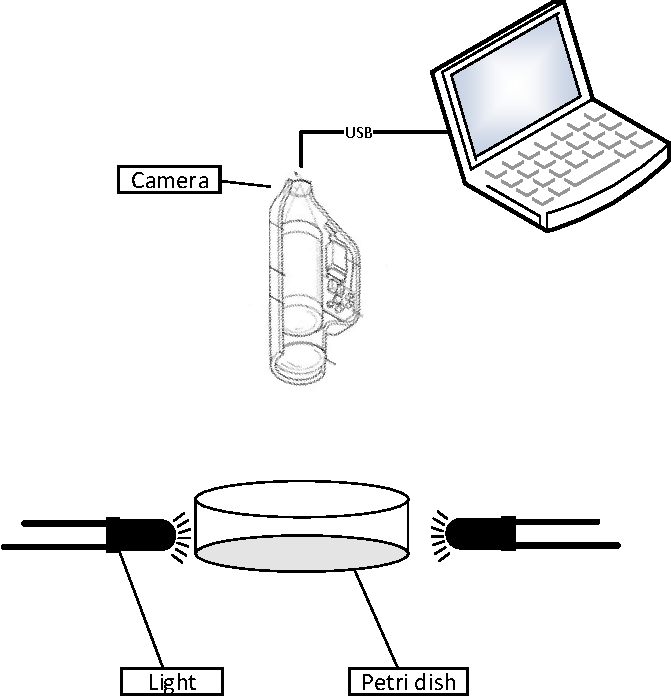
\includegraphics[width=0.6\textwidth]{billeder/software/kameraopstil-crop.pdf}
	\caption{Forsøgsopstilling}
	\label{fig:kameraopstillingen}
\end{figure}
I forsøgsopstillingen anvendtes der i stedet for mikroskopet det indkøbte kamera. En række billeder blev udvalgt til yderligere analyse, hvor Søren Gregersen udpegede hvilke elementer der var øer. På billede \ref{fig:isletSG} er der markeret, hvor en ø er placeret.

\begin{figure}[H]
	\centering
	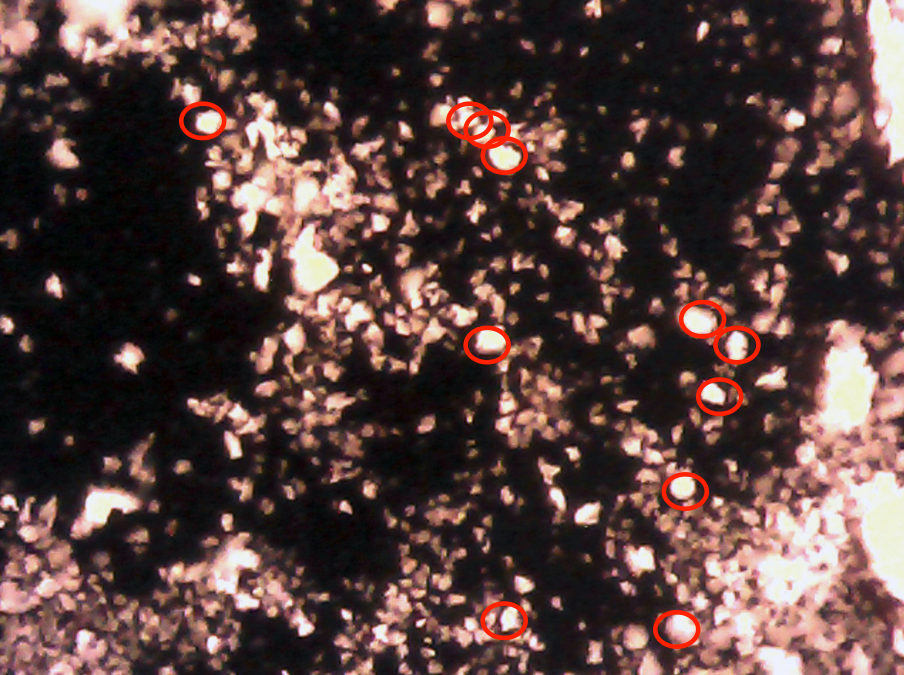
\includegraphics[width=0.6\textwidth]{billeder/software/sgbillede.png}
	\caption{Øer udpeget af Søren Gregersen}
	\label{fig:isletSG}
\end{figure}

Efter nærmere analyse af billederne viste det sig, at det indkøbte kamera ikke var af tilstrækkelig kvalitet til at lave segmentering på billederne. Når øerne blev observeret gennem et almindeligt mikroskop var der langt større kontrast i mellem øerne og det ekstra væv. På billederne fra kameraet findes denne forskel ikke, hvilket udelukker segmentering på denne parameter. Det kan ses på billede \ref{fig:isletSG} at der er områder, hvor lysintensiteten er lige så høj, som de steder hvor øerne er markeret. Dette gør at segmentering på baggrund af lysintensiteten kan udelukkes. Herudover er det tydeligt, at billederne ikke er skarpe nok, hvilket gør at det er svært at vurdere hvad der er øer og ikke øer. De parametre, hvor kameraets kvalitet ikke er tilstrækkelig er derfor bl.a. autoeksponering og autofokus. En bedre styring af autoeksponeringen ville kunne give et bedre kontrast forhold i mellem øerne og det omkringliggende væv, mens en bedre autofokus ville hjælpe på skarpheden i billedet, hvilket muliggøre segmentering baseret på strukturer.

Herudover er der er en polariserende effekt på billederne, hvor nogle af elementerne lyser meget kraftigt op grundet belysningen. Dette gør det er svært at vurdere strukturer og størrelser på elementerne i billedet. 

Efter den første test blev det i samarbejde med vejleder og kunde besluttet, at det indkøbte kamera ikke er af tilstrækkelig kvalitet til at detektere langerhanske øer. I dette system bliver der i stedet udviklet et sæt af billeder, som skal simulere flowet i slangerne. Billederne skal indeholde langerhanske øer, ekstra væv og tilfældig støj for at få dem til at ligne det man observerer gennem et almindeligt mikroskop. Udfra disse billeder skal langerhanske øer detekteres, hvorefter systemet skal åbne ventilen. Billedesættet skal ses som en simulering af kameraet. I en senere prototype vil et kamera af højere kvalitet være påkrævet. Her er det især krav til bedre autoeksponering og autofokus som er essentielle. Dette vil være nødvendigt for at øge kontrasten i mellem øerne og det omkringliggende væv for bedre segmentering. Herudover vil et kamera med polariseringsfilter være en mulighed til at fjerne evt. genskær fra belysningen. Hos Farnell er der andre producenter end det indkøbte Duratool mikroskop, som bl.a. har polariseringsfilter. En test af forskellige kameraer ville være oplagt til at finde det ideelle kamera til optagelse af langerhanske øer. 
\newpage
\subsubsection{Simulering af kamera}
Til at generere et billedsæt, der simulerer langerhanske øer, er der udviklet et Matlab script. Scriptet består overordnet af 3 faser. Den første fase består i at segmentere langerhanske øer udfra et billede og oprette dem som en maske. I anden fase laves en maske bestående af ekstra væv, mens der i tredje fase simuleres flow. I den sidste fase gemmes også de enkelte billeder i formatet .png. De enkelte faser er nærmere beskrevet under deres afsnit. Der anvendes 3 billeder til grundlag for genereringen. Det ene billede viser isolerede øer. Det andet billede viser opløsningen indeholdende øer og ekstra væv. Det sidste billede er et baggrundsbillede uden øer eller ekstra væv. Dette billede anvendes som baggrund for de genererede billeder. Billederne der er valgt stammer fra det indkøbte kamera. Grunden til de kan anvendes som grundlag for genereringen af billeder, på trods af kameraets utilstrækkelige kvalitet, er at øerne og det ekstra væv er adskilt i de enkelte billeder. Dette muliggør en seperat segmentering af øer og væv, som  herefter kan sammensættes til billeder der ligger tæt op af det man observerer gennem et almindeligt mikroskop. De 3 billeder er vist herunder.

\begin{figure}[htbp] \centering
\begin{minipage}[b]{0.3\textwidth} \centering

\includegraphics[width=1.00\textwidth]{billeder/software/1.jpg} % Left picture
\end{minipage} \hfill
\begin{minipage}[b]{0.3\textwidth} \centering
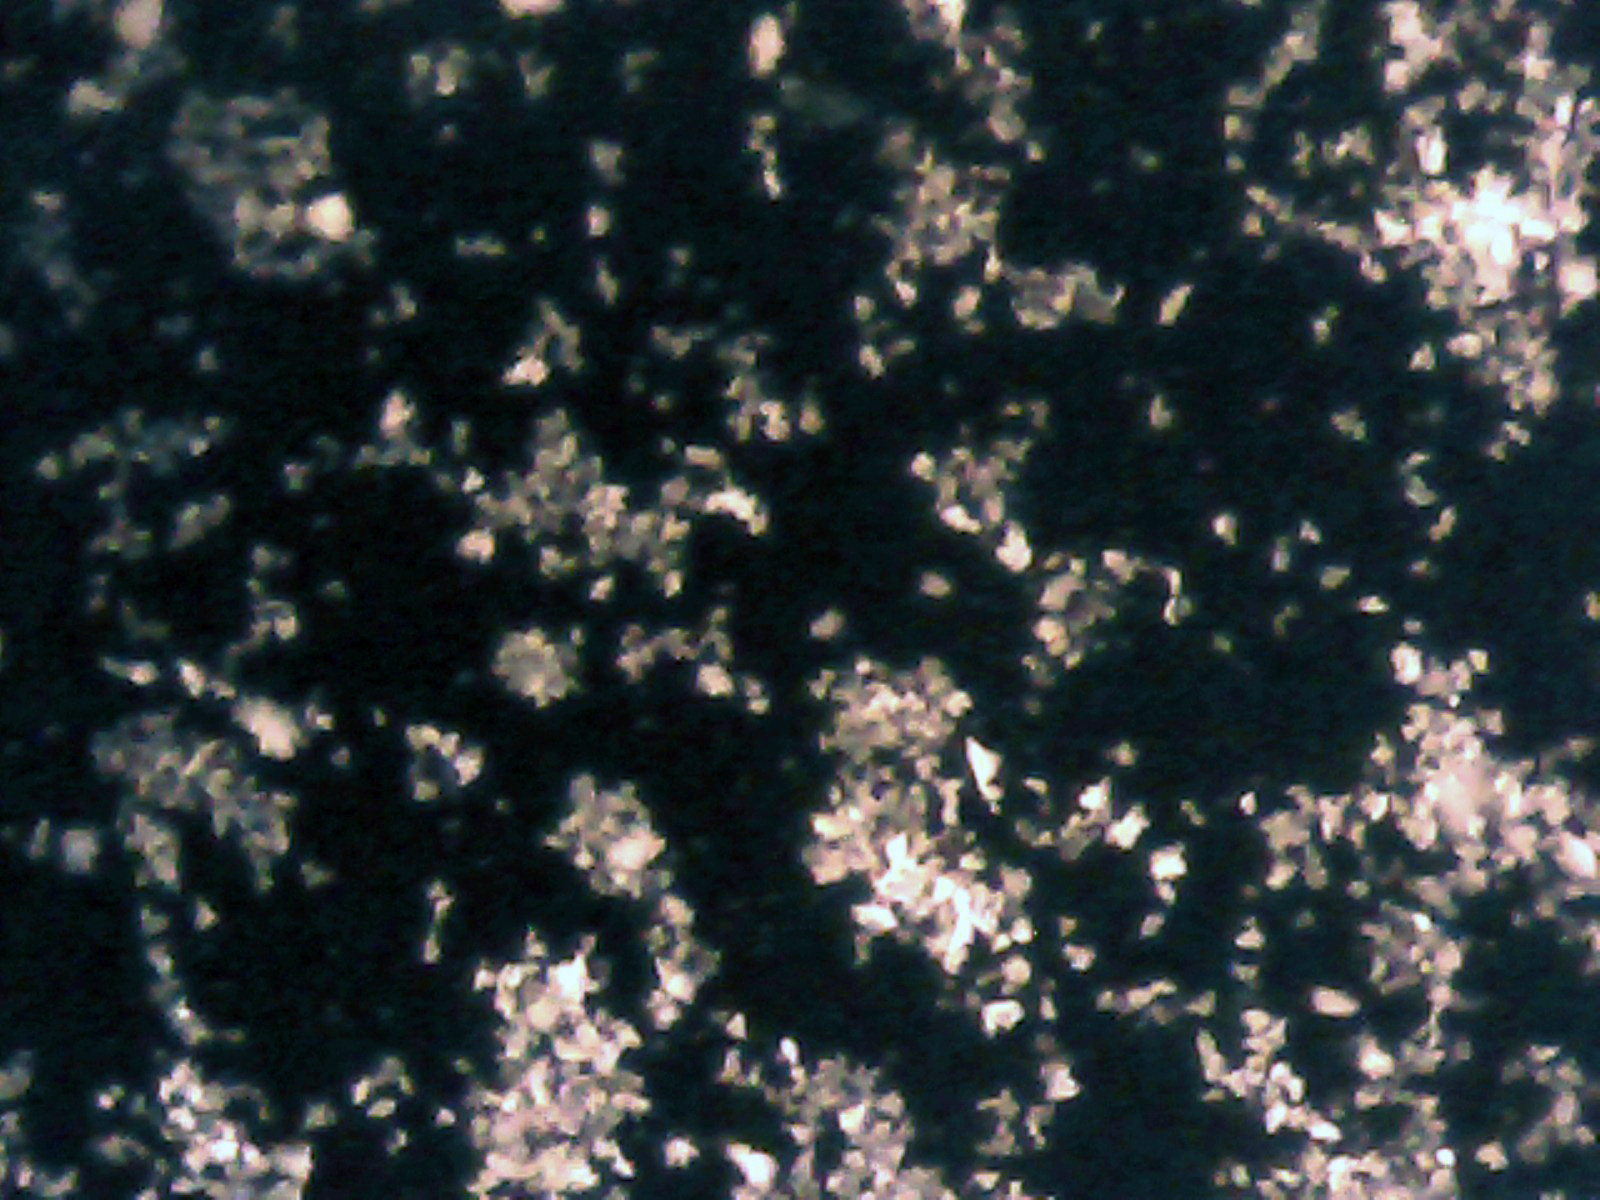
\includegraphics[width=1.00\textwidth]{billeder/software/2.jpg} % Right picture
\end{minipage} 
\hfill
\begin{minipage}[b]{0.3\textwidth} \centering

\includegraphics[width=1.00\textwidth]{billeder/software/3.jpg} % Right picture
\end{minipage} \\  % Captions og labels
\begin{minipage}[t]{0.3\textwidth}
\caption{Billede indeholdende langerhanske øer} % Left caption and label
\label{fig:img1}
\end{minipage} \hfill
\begin{minipage}[t]{0.3\textwidth}
\caption{Billede indeholdende ekstra væv} % Right caption and label
\label{fig:img2}
\end{minipage}
\hfill
\begin{minipage}[t]{0.3\textwidth}
\caption{Baggrundsbillede} % Right caption and label
\label{fig:img3}
\end{minipage}
\end{figure}

\textbf{Fase 1}

Segmenteringen af langerhanske øer sker ud fra billede 1 \ref{fig:img1}, hvor funktionen circleFinder anvendes til at finde centrum og radius på af de fundne celler. Resultatet af circlefinder segmenteringen er vist i fiugr \ref{fig:circlefinder}

 \begin{figure}[H]
	\centering
	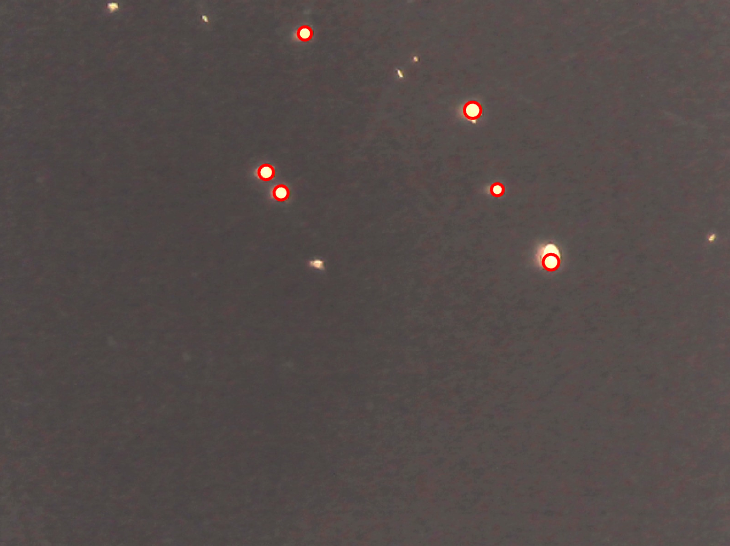
\includegraphics[width=0.5\textwidth]{billeder/software/circlefinder.png}
	\caption{Circlefinder til ø detektion}
	\label{fig:circlefinder}
\end{figure}

Circlefinder funktionen giver følgende funktion, som kan anvendes til at detektere cirkler med. Parametrene Sensitivty og edgeThreshold beskriver, hvor cirkulære objekterne er og generelt hvor følsom algoritmen er. Som det ses på figur \ref{fig:circlefinder} findes der kun én cirkel pr. ønsket ø.
\begin{lstlisting} 
detectCircles = @(x) imfindcircles(x,[12 30], ...
	'Sensitivity',0.8500, ...
	'EdgeThreshold',0.20, ...
	'Method','PhaseCode', ...
	'ObjectPolarity','Bright');
[centers, radii, metric] = detectCircles(im);
\end{lstlisting} 


\textbf{Fase 2}

I anden fase bliver det ekstra væv segmenteret ud fra billede 2 (figur \ref{fig:img2}). Til dette er der anvendt Color Threshold appen i Matlab. Ved hjælp af denne app er der lavet en funktion, som opretter en logisk maske af det ekstra væv. Opsætningen i appen er vist i figur (REF) \fxnote {Indsæt figur}. Yderligere er der anvendt morfologiske operationer til at fjerne uønskede objekter fra masken, samt fjerne støj. Til at fjerne uønskede objekter er funktionen \textit{bwareafilt} anvendt, med parametrene 150 og 500. Dette fjerner alle objekter under 150 og over 500 sammenhørende pixels. Til at udfylde huller i de enkelte objekter er funktionen \textit{imfill} brugt. 

\textbf{Fase 3}

I fase 3 sker selve flow simuleringen. Flowsimuleringen er opbygget på den måde, at den består af henholdvis en sekvens indeholdende en langerhansk ø efterfulgt af en sekvens uden en ø. I selve programmet indlæses et nyt billede hvert 0,1 sekund. Derfor skal der generes en passende mængde billeder, som programmet kan indlæse. Fase 3 er implementeret så der minimum genereres 252 eller maksimalt 432 billeder, hvilket giver en samlet sekvenslængde på 25,2 eller 43,2 sekund. Grunden til at antallet af billeder varierer er at længden af sekvensen uden en langerhansk ø bestemmes udfra en random variabel. Dette gøres for, at simulere at det kan være variabel tid mellem en ny ø kommer i gennem slangen. I scriptet genereres der i alt 18 fulde sekvenser. Det betyder, at der passerer i mellem 25 og 43 øer i minuttet. Antallet af øer der passere pr. minut er bestemt ud fra formel \ref{formular:isletprmin}: 
\begin{align}
\frac{18}{\frac{n}{10}} * 60 = \text{Antal øer pr. minut}
\text{ , hvor n er antallet af billeder i sættet}
\label{formular:isletprmin}
\end{align} 
I figur \ref{fig:boxplot} er vist et boxplot som viser distributionen af hvor mange øer der passere i minuttet. Det ses at medianen ligger over 30 øer pr. minut, hvilket betyder at der i gennemsnit vil komme over 30 øer pr minut. De 30 øer pr. minut stammer fra hastighedskravet fra systemets kvalitetskrav (\ref{subsec:qa}).

 \begin{figure}[H]
	\centering
	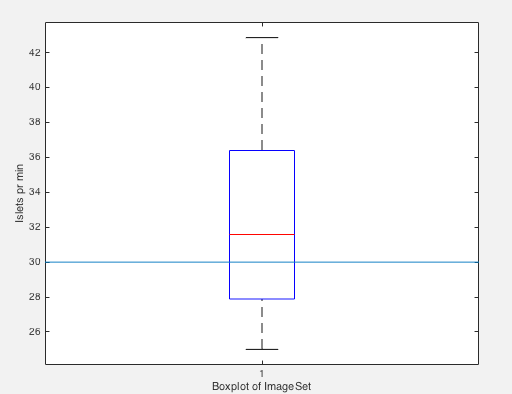
\includegraphics[width=0.5\textwidth]{billeder/software/boxplot.png}
	\caption{Boxplot af distrubutionen af øer pr. minut}
	\label{fig:boxplot}
\end{figure}

Selve flowsimuleringen sker i et for loop. Først udvælges en tilfældig celle ved hjælp af randi (uniform fordelt random variabel). I for loopet opdateres dens center position ud fra 2 variabler (newXPos og newYPos). X positionen springer med et fast interval for hver iteration (160 px). Inden for loopet fastsættes start positionen for cellen med \textit{randi}, som giver et tal mellem 0 og 1200 px (højden på billedet). Herefter opdateres den nye Y position ved hjælp af randn (normal fordelt random variabel) med middelværdi sat til startpositionen og en standard afvigelse på 50 pixels. I figur \ref{fig:flowsim} er flow simulationen illustreret for de i alt 18 sekvenser, med en graf for hver celle. Det ses at cellen flytter sin Y position tilfældigt, mens X positionen springer med et fast interval for hver iteration i for loopet.

\begin{figure}[H]
	\centering
	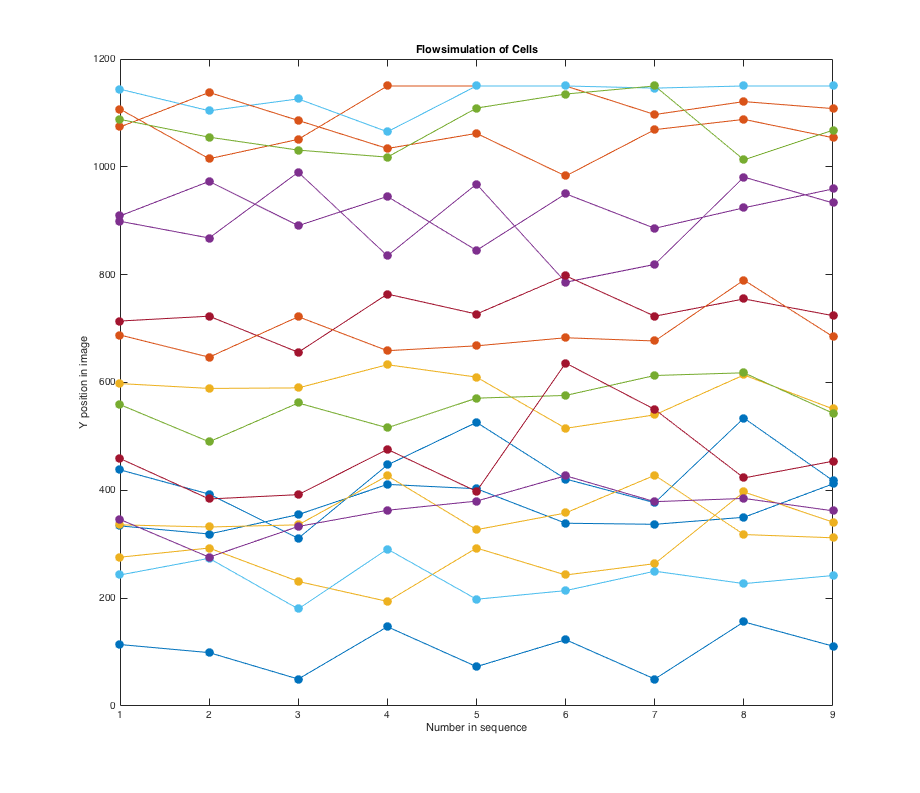
\includegraphics[width=0.5\textwidth]{billeder/software/Simulation.png}
	\caption{Illustration over flow simuleringen}
	\label{fig:flowsim}
\end{figure}

Efter generering af ny x og y position oprettes en maske for cellen ved brug af funktionen createCirclesMask. Til at indsætte cellen i baggrundsbilledet indekseres baggrundsbilledet med masken for cellen, så gråtoneværdierne fra det oprindelige billede indsættes.

Yderligere er der tilføjet tilfældig støj til billedet i form af “Salt and pepper” og gausisk hvid støj. Her er Matlab funktionen \textit{imnoise} anvendt. 

Masken med ekstra væv flyttes for hver iteration med funktionen \textit{circshift}, som bit shifter arrayet cirkulært. Parametrene definerer antallet af rækker og kolonner arrayet skal shiftes.  Antallet af kolonner er fastdefineret til 160 px, mens rækkerne skiftes efter en normalfordelt random variabel med mean på 0 og standard afvigelse på 50 pixels. Nedenstående figur \ref{fig:histfit} viser fordelingen af antallet af rækker der flyttes. På figur \ref{fig:histfit} er der vist markører for standard afvigelsen ($\sigma$) og $2*$standard afvigelsen ($2\sigma$) for hver side af mean. I mellem $-\sigma$ og $\sigma$ er der 68,26 \% sandsynlighed for, at den nye Y position ville ligge inden for dette område. For 2 sd afvigelse ($2\sigma$) er der 95,45 \% for, at den nye Y position vil ligge inden for dette område.

\begin{figure}[H]
	\centering
	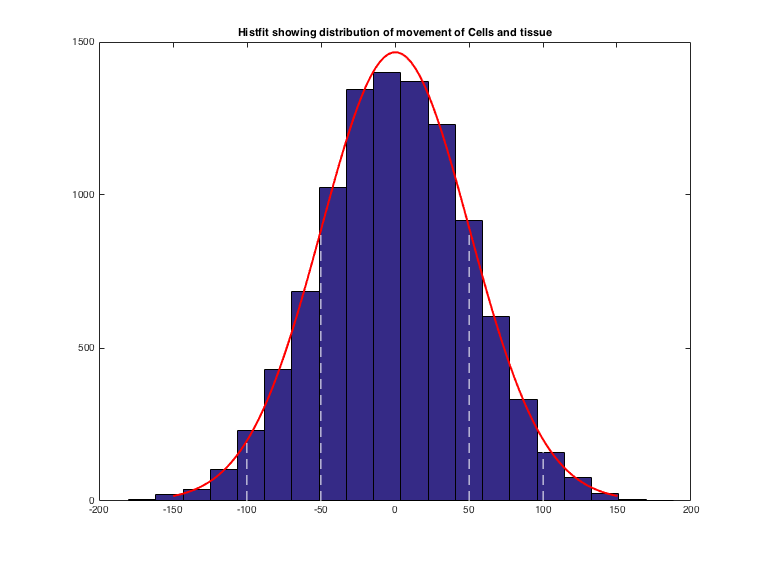
\includegraphics[width=0.5\textwidth]{billeder/software/histfit.png}
	\caption{Histogram over fordelingen af ny Y position}
	\label{fig:histfit}
\end{figure}

Det endelige resultat af billedegeneringen er vist i figur \ref{fig:finalresult}. Til at illustrere hvordan øen flytter sig er der tilføjet en graf, som viser hvordan dens position ændres for hver iteration. Cellen er markeret med en rød ring på billedet.

\begin{figure}[H]
	\centering
	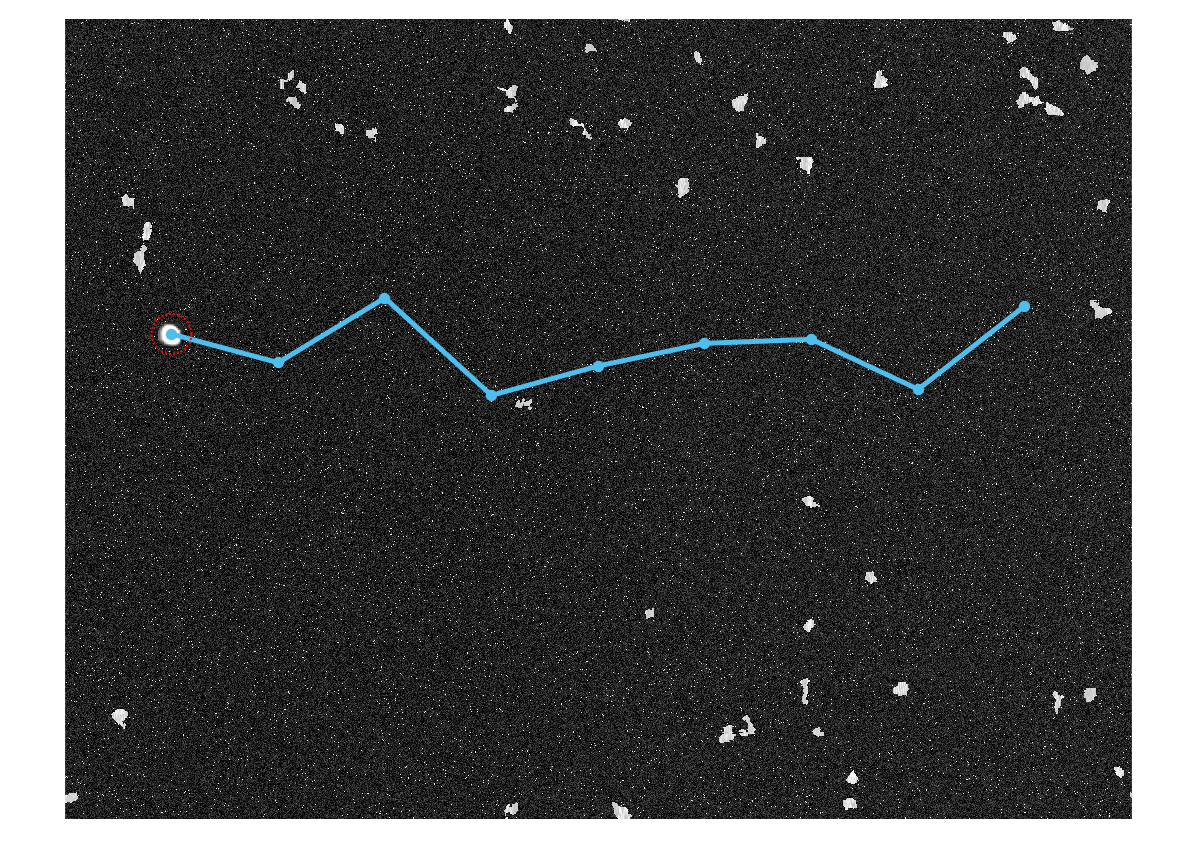
\includegraphics[width=0.7\textwidth]{billeder/software/final.png}
	\caption{Endelige resultat for flowsimulering}
	\label{fig:finalresult}
\end{figure}

Implementeringen af scriptet er vedlagt i bilag \fxnote{Indsæt referencer til bilag}

\newpage
\subsection{Matlab funktioner}
I dette afsnit er implementeringen af de enkelte funktioner i Matlab nærmere beskrevet. Selve implementeringen tager udgangspunkt i beskrivelserne fra design dokumentet. %Herudover er der beskrevet test af de enkelte funktioner.  


\subsubsection{initArduino}
I denne funktion opsættes og initialiseres Arduinoen. Til dette anvendes funktionen \textit{Arduino}, fra Arduino Support pakken. Som parameter til funktionen angives port navnet og board typen (i dette system en Arduino Uno). Arduino variablen gemmes herefter i handles, som en variabel.

Herudover opsættes Arduinoens input og output i funktionen. \fxnote{Mangler beskrivelse}

Selve initialiseringen sker i et try/catch statement, hvis Arduinoen ikke kan initialiseres åbnes en dialogboks (figur: \ref{fig:initArduino}), hvor operatøren kan vælge om systemet skal forsøge at oprette forbindelse igen. 

\begin{figure}[H]
	\centering
	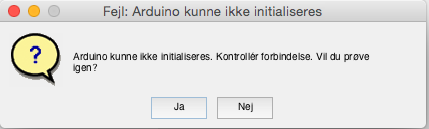
\includegraphics[width=0.5\textwidth]{billeder/software/initArduino.png}
	\caption{Dialogboks til systembesked}
	\label{fig:initArduino}
\end{figure}

Implementeringen af initArduino er vist i nedenstående kode.
\begin{lstlisting} 
while true
    % Try/Catch statement
    try
        % Initialize Arduino and save variable in handles
        handles.a = arduino('/dev/cu.usbmodem1411','Uno');
        % If succes - break while loop
        break
    catch
    % Open quest dialog to inform operator that inializing failed    
    choice = questdlg('Arduino kunne ikke initialiseres. Kontroller forbindelse. Vil du proeve igen?','Fejl: Arduino kunne ikke initialiseres', 'Ja','Nej','Ja');

        switch choice
            % Do nothing - retry inializing again
            case 'Ja'
        
            % Returns to end function
            case 'Nej'
            return
        end
    end
end
\end{lstlisting} 

\subsubsection{cameraFeed}
Denne funktion er implementeret udfra beskrivelsen i designdokumentet. Ref. Dog er den ændret i forhold til ikke at modtage et feed fra kameraet, men i stedet indlæses et billede fra en prædefineret mappe. 
Funktionen har handles som input og output. 

I et while loop itereres der gennem mappen, hvor en counter variabel definerer hvilket billede der skal indlæses. Efter dette nedskaleres billedet til halv størrelse med imresize. Billedet gives herefter som parameter til funktionen detectIslet (REF). I while loopet kaldes der til sidst pause(0,1), som pauser while loopet i 0,1 sekund. Dette simulerer at kameraet optager med 10 f/s. 

Matlab implementeringen er vedlagt i bilag \fxnote{REF}

%\subsubsection{detectIslets}
\newpage
\subsubsection{detectIslets}
\label{subsub:IMdetectIslets}
I denne funktion sker selve billedesegmenteringen af de langerhanske øer. Selve segmenteringen sker via en række morfologiske operationer, som er nærmere beskrevet i dette afsnit. For at illustrere effekten af de enkelte steps er der i løbet af afsnittet vist billeder.

I figur \ref{fig:im} er det oprindelige billede vist. Billedet danner udgangspunktet for selve segmenteringen. Billedet indeholder én langerhansk ø. 

%\begin{lstlisting} 
% Converts the image to logical, based on threshold. 0.72 indicates pixels
% with luminance level above 0,72 (255*0.72 = 183) is converted to a 1. Pixels below this 
% level is converted to 0 
%bw = im2bw(im,0.72);
%\end{lstlisting} 

\begin{figure}[H]
	\centering
	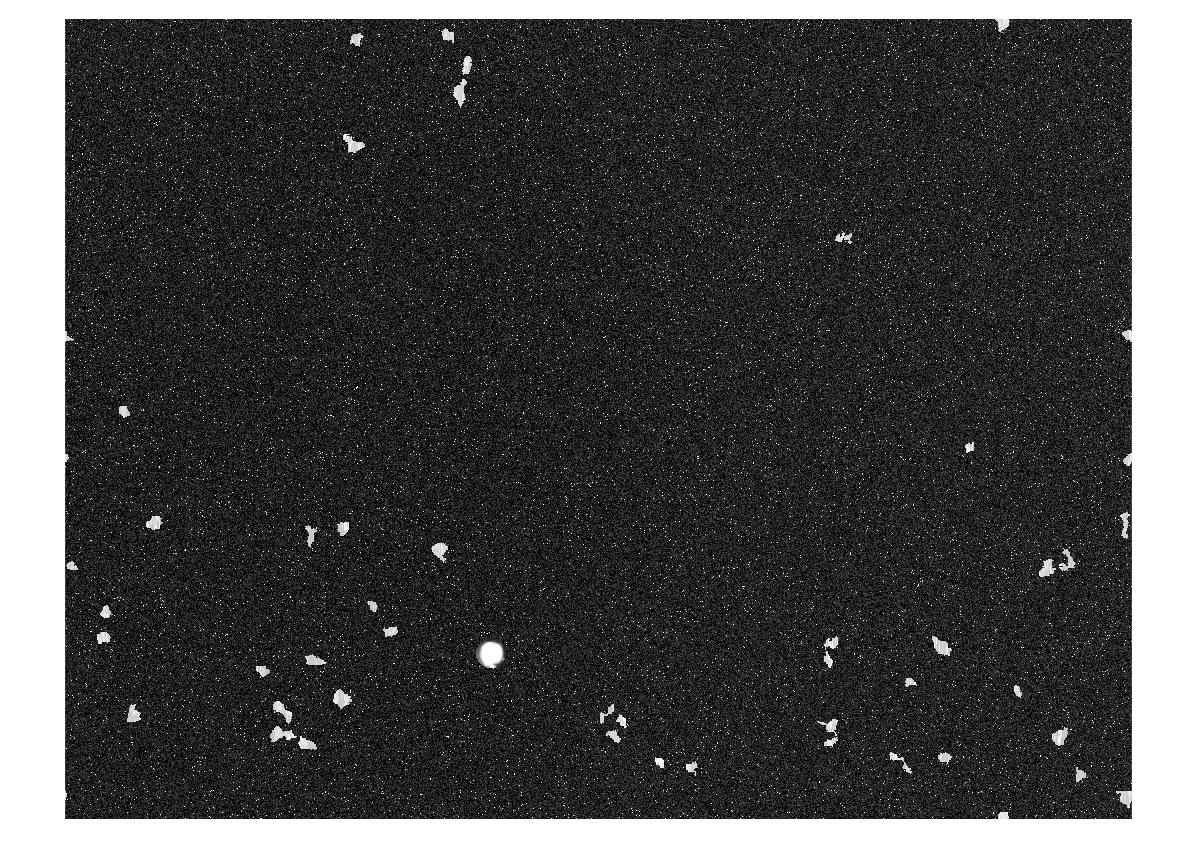
\includegraphics[width=0.6\textwidth]{billeder/software/im.png}
	\caption{Oprindelige billede}
	\label{fig:im}
\end{figure}

Første step af billedesegmenteringen består i, at konvertere det oprindelige billede (\ref{fig:im}) til en logisk maske. Til dette er Matlab funktionen \textit{im2bw} anvendt. 
Effekten af im2bw er vist i figur \ref{fig:im2bw}. Funktionen konvertere alle pixels med en lysstyrke over det angivne threshold (0,72) med 1, og pixels under med 0. Input billedet er et 8 bit billede, dermed indikerer et threshold på 0,72, at pixel værdien skal være over 183 for at blive inkluderet i masken. I nedenstående kode er implementeringen vist.

\begin{lstlisting} 
% Converts the image to logical, based on threshold. 0.72 indicates pixels
% with luminance level above 0,72 (255*0.72 = 183) is converted to 1. Pixels below this 
% level is converted to 0 
bw = im2bw(im,0.72);
\end{lstlisting} 

\begin{figure}[H]
	\centering
	
\includegraphics[width=0.6\textwidth]{billeder/software/im2bw.png}
	\caption{Billede konverteret til logisk}
	\label{fig:im2bw}
\end{figure}

I næste step bliver unødigt støj fra masken fjernet. Til dette anvendes funktionen \textit{bwareaopen}. Denne fjerner alle objekter i masken under 100 sammenhørende px. Dette fjerner de mindste støjkomponenter fra billedet. Effekten af denne funktion er vist i figur \ref{fig:bwarea}. Herudover kaldes funktionen bwlabel, som indeksere hvert af de sammenhørende objekter i masken. Dermed får hvert objekt i figur \ref{fig:bwarea} et unikt index fra 1 til 5. 
\begin{lstlisting} 
% Removes all objects below 100 connected pixels
bw = bwareaopen(bw,100);

% Label connected components
L = bwlabel(bw);
\end{lstlisting} 

\begin{figure}[H]
	\centering
	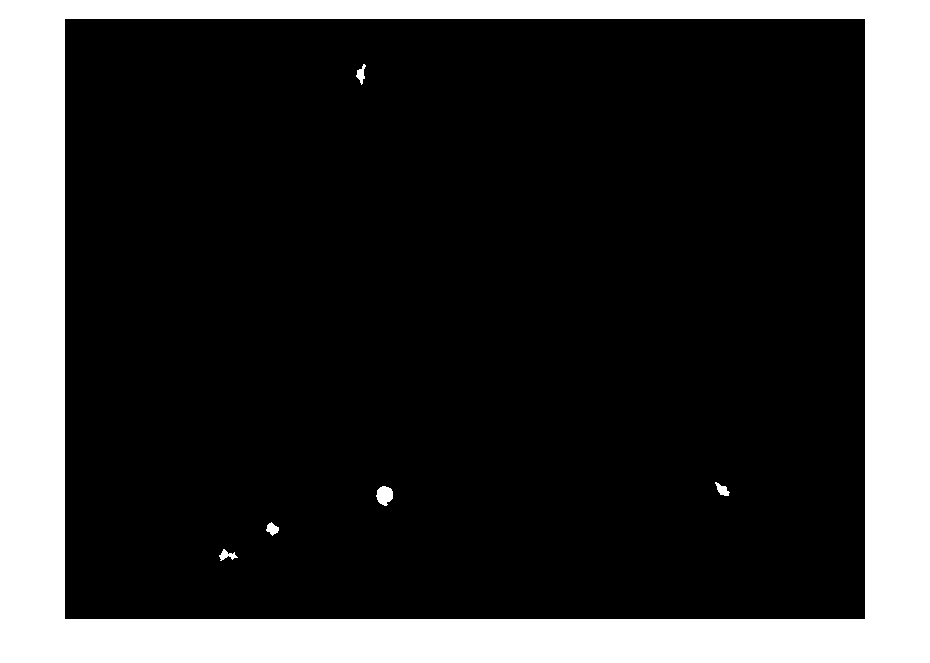
\includegraphics[width=0.6\textwidth]{billeder/software/bwarea.png}
	\caption{Små objekter fjernet}
	\label{fig:bwarea}
\end{figure}

I næste step sker selve ø detekteringen. Detektionen baseres på, at øerne har en mere cirkulær form end resten af vævet. Derfor hentes der egenskaber fra objekterne i masken vha. matlab funktionen \textit{regionsprops}. De egenskaber der hentes er med til, at beskrive hvor cirkulært objektet er. De egenskaber som hentes er arealet, center positionen, omkredsen og excentriciteten. Excentriciteten beskriver hvor langstrakt objektet er. Hvis excentriciteten er 0 er det en perfekt cirkel mens det vil være en langstrakt ellipse hvis værdien er 1.

Udfra arealet og omkredsen af objekterne anvendes de 2 nedenstående formler til bestemmelse af 2 værdier for radiusen af objektet:
\begin{align}
Areal = R1^2*\pi => R1 = \sqrt{\frac{\text{Areal}}{\pi}}
\end{align}
\begin{align}
Omkreds = 2*R2*\pi => R2 = \frac{\text{Omkreds}}{2*\pi}
\end{align}

Udfra disse 2 radius værdier, vil det objekt, hvor der er mindst forskel i mellem de 2, være det objekt der er mest cirkulært. Til at illustrere dette er der i figur \ref{fig:circleelip} vist en cirkel og en ellipse begge med samme areal. Udfra \textit{regionsprops} og de 2 formler for radius kan der bestemmes 2 radiuser for henholdsvis cirklen og ellipsen. Forskellen bestemmes ved, at trække de 2 beregnede værdier fra hinanden. I udregningerne nedenfor er den første kolonne værdier for cirklen, mens den anden er for ellipsen. Som det ses er forskellen mindst ved cirklen, hvilket indikerer, at den er mest cirkulær.
  
\begin{lstlisting} 
r1 =  100.0017   99.9380

r2 =  99.7978  105.7890

rDif = 0.2039    5.8510
\end{lstlisting} 

\begin{figure}[H]
	\centering
	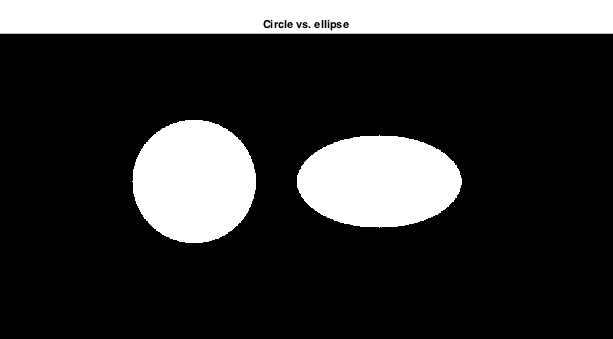
\includegraphics[width=0.6\textwidth]{billeder/software/circleellipse.png}
	\caption{Cirkel sammenlignet med ellipse}
	\label{fig:circleelip}
\end{figure}

Indekset for det objekt med mindst forskel i radius og indekset for det objekt med den mindste excentricitet gemmes i variabler. I nedenstående kode er det vist, hvordan dette er implemeneteret i Matlab.

\begin{lstlisting} 
stats = regionprops(bw,'Area','Centroid','Perimeter','Eccentricity');

r1 = sqrt([stats.Area]/pi);
r2 = [stats.Perimeter]/(2*pi);
% The absolute difference between the 2 radius is calculated
rDif = abs(r1-r2);
% The index of the lowest difference is returned
[~, idx] = min(rDif);
% The index of the object with the lowest eccentricity is returned 
[~, idx2] = min([stats.Eccentricity]);
\end{lstlisting} 

\newpage
I det sidste step i segmenteringen af den langerhanske ø kontrolleres det om radius forskellen og excentricitet ligger under nogle fast definerede grænseværdier. Værdierne er fundet ved, at analysere en række billeder og deres objekters radius og excentricitet. Radius og excentriciteten bliver gemt i logfilen, så de kan analyseres for senere at justere grænseværdierne. Hvis objektets værdier er under disse grænseværdier er en ø detekteret. Når en ø er detekteret illustreres det med en grøn ring på GUI. Til dette er funktionen \textit{viscircles} anvendt, hvor center positionen og radius for objektet anvendes. 

For at løse udfordringen med, at den samme ø vil optræde på det næste billede, er der implementeret et smalt detekteringsvindue (100 pixels bredt). Når øen er detekteret inden for dette område bliver variablen isletDetected sat til true. Denne variabel anvendes til styring af ventilen. Implementingen af dette er vist i nedenstående kode.


\begin{lstlisting} 
% If the difference between radius AND eccentricity is below the defined
 % values an islet has been detected
 if rDif(idx) < 0.45 && stats(idx2).Eccentricity <0.51
     
 % Show circle of cell on the 2 axes
 viscircles(h,stats(idx2).Centroid,r1(idx2)+10,...
 'LineStyle','-','edgecolor','g','LineWidth',1,'DrawBackgroundCircle',...
 false);
 viscircles(s,stats(idx2).Centroid,r1(idx2)+10,...
 'LineStyle','-','edgecolor','g','LineWidth',1,'DrawBackgroundCircle',...
 false);

     
      % Detection window  (0 to 100 pixels)
      if stats(idx2).Centroid(1) <=100 
      handles.flag1 = true;
      handles.count = handles.count+1; 
      set(handles.txtIslets,'String',num2str(handles.count));
      handles.isletDetected = true;
      end
\end{lstlisting} 

Figur \ref{fig:segmented} viser slutresultatet af segmenteringen, hvor masken kun indeholder den langerhanske ø fra det oprindelige billede. 


\begin{figure}[H]
	\centering
	
\includegraphics[width=0.6\textwidth]{billeder/software/segmented.png}
	\caption{Slutresultat af segmentering}
	\label{fig:segmented}
\end{figure}

\newpage
I figur \ref{fig:finalimage} er det oprindelige billede vist, med markering af den detekterede ø.


\begin{figure}[H]
	\centering
	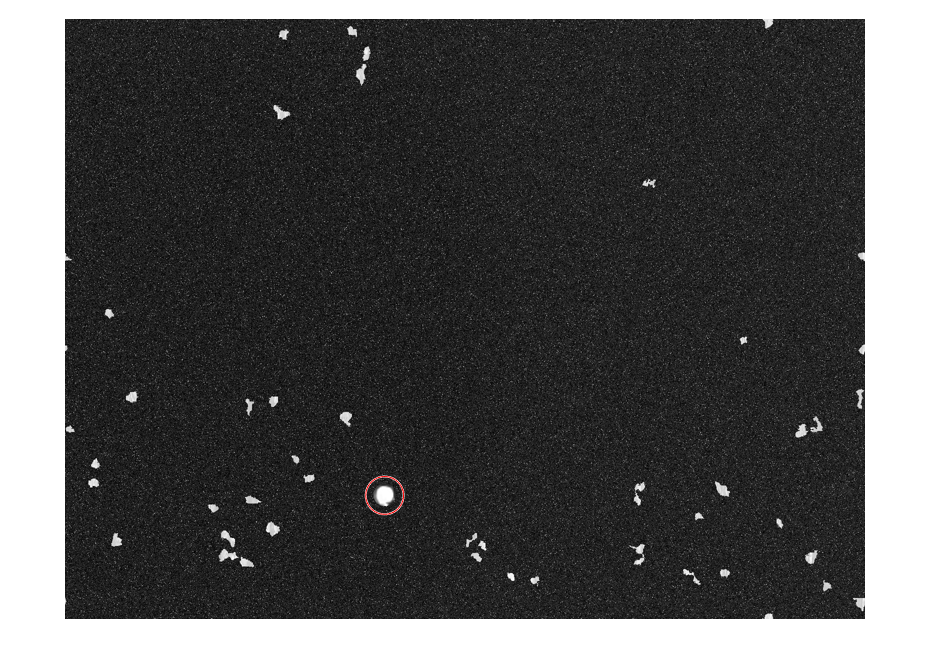
\includegraphics[width=0.6\textwidth]{billeder/software/finalimage.png}
	\caption{Oprindelige billede med detekteret ø}
	\label{fig:finalimage}
\end{figure}

\newpage
\textbf{Test af billedeprocessering}

En udfordring med billedeprocesseringen er, at hastigheden ikke må være for langsom i forhold til frameraten for kameraet. Som beskrevet under funktionen cameraFeed (\ref{subsub:camfeed} indlæses et nyt billede hvert 0,1 sekund. Billedeprocesseringen skal dermed være hurtigere end dette for at følge med. Til test af dette er Matlab funktionen tic/toc anvendt, som måler hvor langt tid billedprocessingen tager om at eksekvere. I figur \ref{fig:dataprocess} viser grafen hvor lang tid det har taget, at behandle de enkelte billeder. Den røde streg viser den gennemsnitlige tid for processeringen. For den nuværende implementering tager billedeprocessingen 0,0104 sekund pr. billede, hvilket er indenfor grænsen på 0,1 sekund. Tiden vil variere alt efter tilgængelig processorkraft og om der skal udføres andre opgaver, eksempelvis opdatere figurer på GUI. 

\begin{figure}[H]
	\centering
	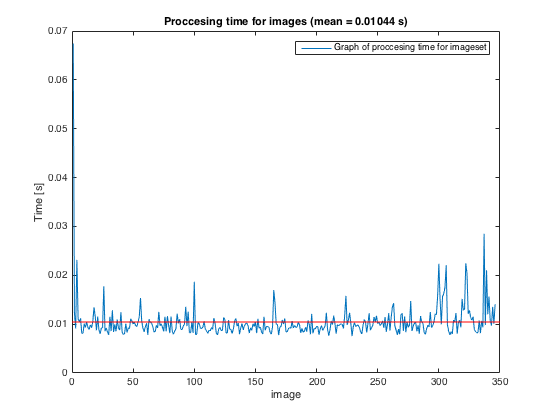
\includegraphics[width=0.6\textwidth]{billeder/software/dataprocessing_2.png}
	\caption{Test af tidsforbrug for billedeprocessering}
	\label{fig:dataprocess}
\end{figure}
 
\newpage
\subsubsection{loadCell}
Funktionen til load cellen er implementeret efter beskrivelsen i design dokumentet. Dens funktion er, at konvertere det analoge input (v) til indholdet (ml) i celleopløsningsbeholderen. Dette er implementeres ved en liniær model:
\begin{align}
mL = a*input+b \text{, hvor a er hældningen og b er skæringen med y aksen}
\end{align}
Det analoge input ganges altså med en faktor a plus et offset b for at konvertere spænding til antal ml. Nedenstående tabel viser indgangsspændingen for forskellige mængder i beholderen. Udfra disse data er der lavet en liniær regression for at finde hældningen a og skæringen b.
\begin{center}
		\begin{longtable}{ | m{3cm} | m{3cm}| } 
			\hline
			\textbf{ml i beholder} &\textbf{Analog input} \\ 
			\hline
			 \SI{0}{\milli\litre} & \SI{0}{\volt} \\ 
			\hline
			 \SI{25}{\milli\litre} & \SI{0}{\volt} \\ 
			\hline
			\SI{50}{\milli\litre} & \SI{0}{\volt} \\ 
			\hline
			\SI{75}{\milli\litre} & \SI{0}{\volt} \\ 
			\hline
			\SI{100}{\milli\litre} & \SI{0}{\volt} \\ 
			\hline
			\SI{125}{\milli\litre} & \SI{0}{\volt} \\ 
			\hline
			\SI{150}{\milli\litre} & \SI{0}{\volt} \\ 
			\hline
			\SI{175}{\milli\litre} & \SI{0}{\volt} \\ 
			\hline
			\SI{200}{\milli\litre} & \SI{0}{\volt} \\ 
			\hline
			\SI{225}{\milli\litre} & \SI{0}{\volt} \\ 
			\hline
			\SI{250}{\milli\litre} & \SI{0}{\volt} \\ 
			\hline
			\caption{Kalibreringsdata for loadcellen}
			 		\end{longtable}
\end{center}

Figur REF viser den liniære funktion, samt de enkelte data punkter fra tabellen. I Matlab er funktionen .. anvendt til at finde det bedste liniære fit. Regressionen er baseret på Least Square metoden. \fxnote{Henvisning}
Udfra beregningerne i Matlab er hældningen a og skæringen b fundet til hhv:
\begin{align}
a = something
b = something
\end{align}
Den endelige funktion er dermed givet ved:
\begin{align}
ml = something*input+something
\end{align}

For at reducere støj og mindske følsomheden overfor hurtigere ændringer i indgangsspændingen er der implementeret en midling af de sidste 10 målinger. Dette gør konverteringen mere robust overfor støj.  


\subsubsection{valveControl}
I denne funktion styres åbning og lukning af ventilen. Til dette anvendes funktionen writeDigital
\subsubsection{pumpControl}

\subsubsection{settings}
\subsubsection{exportData}

\newpage
\subsection{GUI}
\subsubsection{Hovedvindue}
Screenshot af det færdige program

Beskrivelse
\subsubsection{Indstillingsvindue}
Screenshot af Indstillingsvindue

Beskrivelse

\newpage
\subsection{Matlab callbacks}
Dette afsnit beskriver callback funktionerne..
%\subsubsection{•}
\subsubsection{Start callback}

\subsubsection{Stop callback}

\subsubsection{Settings callback}